% !Mode:: "TeX:UTF-8"
\documentclass[bachelor,openany,oneside,color,AutoFakeBold=true]{buaathesis}

\graphicspath{{images/}}

\usepackage{xcolor}
\hypersetup{
    colorlinks,
    linkcolor={black},
    citecolor={blue!50!black},
    urlcolor={blue!80!black}
}

% 参考文献
\usepackage{gbt7714}
% 参考文献输出方式,numerical为按照出现顺序,authoryear为按照作者姓名和年份
\citestyle{numerical}
% \citestyle{authoryear}

\begin{document}

% 用户信息
% !Mode:: "TeX:UTF-8"

% 学院中英文名,中文不需要“学院”二字
% 院系英文名可从以下导航页面进入各个学院的主页查看
% https://www.buaa.edu.cn/jgsz/yxsz.htm
\school
{计算机}{(School of Computer Science and Engineering)}

% 专业中英文名
\major
{计算机科学与技术}{Computer Science and Technology}

% 论文中英文标题
\thesistitle
{Speculative Decoding with Big Little Decoder}
{}
{Speculative Decoding with Big Little Decoder}
{}

% 作者中英文名
\thesisauthor
{刘伟哲}{Liu Weizhe}

% 导师中英文名
\teacher
{黄迪}{Huang Di}
% 副导师中英文名
% 注:慎用‘副导师’,见北航研究生毕业论文规范
%\subteacher{(副导师姓名)}{(Name of Subteacher)}

% 中图分类号,可在 http://www.ztflh.com/ 查询
\category{T}

% 本科生为毕设开始时间;研究生为学习开始时间
\thesisbegin{2024}{6}{1}

% 本科生为毕设结束时间;研究生为学习结束时间
\thesisend{2024}{5}{27}

% 毕设答辩时间
\defense{2024}{5}{27}

% 中文摘要关键字
\ckeyword{自然语言处理,推理加速,解码器,推测性解码}

% 英文摘要关键字
\ekeyword{NLP, Inference accelera, decoder}

% !Mode:: "TeX:UTF-8"

% 班级
\class{210613}

% 学号
\studentID{21371421}

% 单位代码
\unicode{2106}

% 论文时间,用于首页
\thesisdate{2024}{5}


% 任务书信息
\include{data/bachelor/assign}

% 页眉页脚样式
\pagestyle{mainmatter}
% 封面、任务书、声明
\maketitle
% 摘要
% !Mode:: "TeX:UTF-8"

% 中英文摘要
\begin{cabstract}
    基于 Transformer 架构的大语言模型(Large Language Model, LLM)使自然语言处理领域取得了巨大进步。然而,由于这些模型的推理延迟较长,它们在各种实时应用中的使用受限。自回归生成任务进一步加剧了推理延迟,因为模型需要迭代运行,按顺序生成标记,不能利用标记级并行化。为了解决这个问题,该文提出了Big Little Decoder(BiLD)框架,它可以在不降低生成质量的前提下提高推理效率,适用于各种文本生成应用。BiLD 框架包含两个不同大小的模型,它们协同生成文本。小模型以自回归方式运行,以较低的推理成本生成文本;大模型偶尔以非自回归方式修正小模型的不准确预测。为了协调大小模型,BiLD 引入了两种简单而有效的策略:(1) Fallback 策略用于确定何时将控制权移交给大模型;(2) Rollback 策略用于确定大模型如何修正小模型不准确的预测。在实验评估部分,BiLD 应用于各种文本生成场景,包括 IWSLT 2017 De-En 和 WMT 2014 De-En 上的机器翻译,以及 XSUM 和 CNN/DailyMail 上的摘要生成。在 NVIDIA T4 GPU 上,在几乎不减低生成质量的前提下,BiLD 实现了高达 2.12 倍的速度提升。此外,BiLD 框架完全即插即用,无需修改训练过程或模型架构。
\end{cabstract}

% \begin{eabstract}
% Here is the Abstract in English. And this is a test sentence, just for
% a test to see how the buaathesis works. You can just ignore this.\par
% This is another pargraph.
% \end{eabstract}
% 目录
\tableofcontents

% 正文页码样式
\mainmatter

% 正文
% !Mode:: "TeX:UTF-8"
\chapter{研究背景}

近年来,Transformer 已成为各种自然语言处理任务的主流模型。LLM 的出现进一步提升了 Transformer 架构的潜力。LLM 在海量文本语料库中训练得到数千亿个参数,模型质量卓越。但是由于其规模过大,高效运行模型进行推理十分困难,这限制了大语言模型在实时响应任务中的应用。

\section{相关工作}
为了提高 Transformer 推理速度并降低推理成本,前人探索了高效架构设计\upcite{iandola2020squeezebert}、量化\upcite{kim2021ibert}、剪枝\upcite{gale2019state}和神经架构搜索\upcite{chen2021adabert}。

部分研究致力于高效解码机制。非自回归解码\upcite{gu2018nonautoregressive}通过并行生成多个输出标记避免文本串行化生成,提升推理速度,但是质量较差。后续研究在此基础上通过添加辅助信息或多次迭代进一步改进推理质量。此外,也有研究降低解码器深度,同时增加编码器深度\upcite{kasai2021deep}或执行早期退出(early exiting)\upcite{schuster2022confident}。这些工作都需要修改模型结构和训练流水线。

另一方面,可以使用多个模型提升推理效果。知识蒸馏\upcite{hinton2015distilling}通过训练较小模型来学习较大模型的行为,从而提高模型性能。集成学习\upcite{pai-2020-qiaoning}对多个模型进行独立训练,然后将它们的预测结果结合起来,以提高整体性能。

与本文工作最相关的是,使用强模型对弱模型进行评分和推测性采样,提供强模型的概率分布的无偏估计器,从而加速推理\upcite{pmlr-v202-leviathan23a,chen2023accelerating}。实验评估表明,本文的方法由于采用了非随机回滚策略、动态回退窗口大小、预测对齐,可以提供更优越的生成质量和推理速度权衡。

% !Mode:: "TeX:UTF-8"

\chapter{问题描述}

大模型的推理速度慢,限制了它的实时应用。这样的低效推理在自回归生成任务(机器翻译、文本总结、语言模型等)中尤为显著。自回归生成任务需要多次迭代运行,每个标记(token)的生成都依赖于之前生成的标记序列。推理过程串行化,推理过程的内存带宽受限,硬件利用率差,推理速度慢。

在自回归生成任务中的第 $n$ 轮解码迭代中,小模型和大模型分别将已经生成的文本 $y_{1:n-1}=(y1,\dots,y_{n-1})$ 作为输入,生成下一个标记的概率分布 $p_S(y|y_{1:n-1})$ 和 $p_L(y|y_{1:n-1})$。

\begin{align}
    y_{n,S} & \sim p_S(y|y_{1:n-1}) \\
    y_{n,L} & \sim p_L(y|y_{1:n-1})
\end{align}

仅当小模型可能作出不准确预测时,才需要大模型生成文本,该判别函数为$\pi(y_{1:n-1})$:

\begin{equation}
    y_n= \begin{cases}y_{n, S} & \text { if } \pi\left(y_{1: n-1}\right)=0 \\ y_{n, L} & \text { if } \pi\left(y_{1: n-1}\right)=1\end{cases}
\end{equation}

为了提高推理速度,需要设计一个轻量的判别函数 $\pi$,只在必要时使用大模型。

当大模型接管控制权并预测标记 $y_n$ 时,它可以并行接收多个输入标记 $y_{1:n-1}$,实现非自回归并行推理。这样虽然没有减少浮点运算量(FLOP),但是提高了解码过程的算术强度和硬件利用率,实现了推理加速。

\chapter{研究方法}

Big Little Decoder(BiLD)\upcite{kim2023speculative} 框架由 2 个解码器模型(大模型和小模型)组成,它们协同工作生成文本序列。其中,小模型运行开销小,自回归地生成大部分文本。大模型偶尔修正小模型不准确的预测,执行高效的非自回归运算。与常规的自回归执行相比,这种自回归小模型、非自回归大模型结合的方案大大提升了推理速度,最高可达原来的 2 倍,同时保持了类似或更好的生成质量。BiLD 框架可应用于各种文本生成场景,除了添加小模型外,无需进行额外的训练或修改现有的模型架构。

\begin{figure}[htbp]
    \centering
    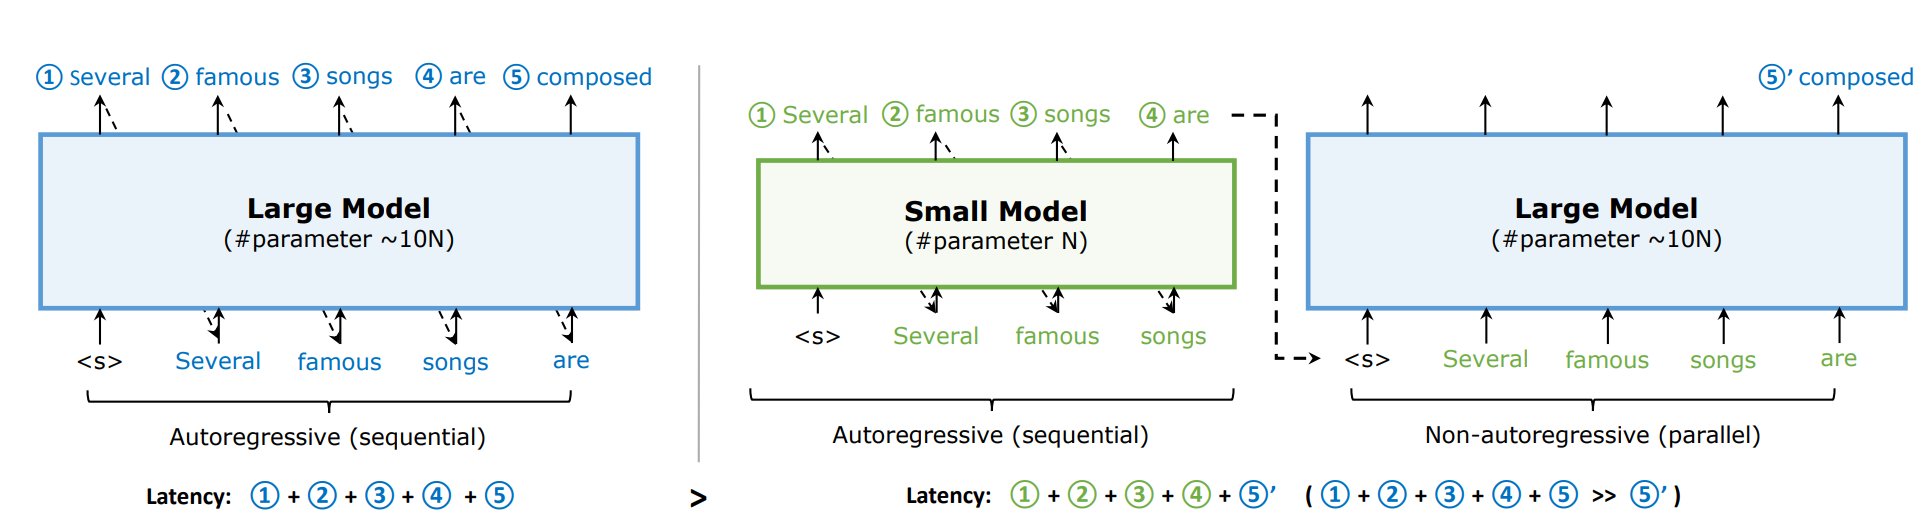
\includegraphics[width=0.9\textwidth]{BiLD.png}
    \caption{
        大模型的正常自回归解码流程(左);BiLD 解码流程(右)。在 BiLD 中,小模型自回归地生成标记,直到将控制权移交给大模型。 然后,大模型将小模型并行生成的标记作为输入,非自回归(即并行)地生成下一个标记。这样可以更有效地利用底层硬件,从而提升推理速度。
    }
    \label{fig:BilD}
\end{figure}

\section{可行性分析}

在多数文本生成场景中,只要纠正了部分错误预测,比大模型小一个数量级的模型也能达到与大模型相当的生成质量。为了验证这一说法,评估两种不同的生成场景:在 WMT 2014 De-En\upcite{bojar-etal-2014-findings} 上使用 mT5\upcite{xue2021mt5} 进行机器翻译,在 CNN/DailyMail\upcite{NIPS2015_afdec700} 上使用 T5\upcite{DBLP:journals/corr/abs-1910-10683} 进行摘要生成。通过控制阈值调整大模型的比重,统计大模型和小模型预测同一标记的似然性。

图~\ref*{fig:Motivating} 显示了在 2 个基准验证数据集上不同比例的大模型参与时的文本生成质量。结果表明,当大模型替代了小模型约 20\% 的不准确预测时,规模仅大模型 $1/10$ 的小模型可以保持大模型的生成质量。虽然这个实验假定大模型的预测在每次迭代中都是准确的,但它仍然证明了在保持小模型低推理延迟的同时实现大模型文本生成质量的可行性。

\begin{figure}[htbp]
    \centering
    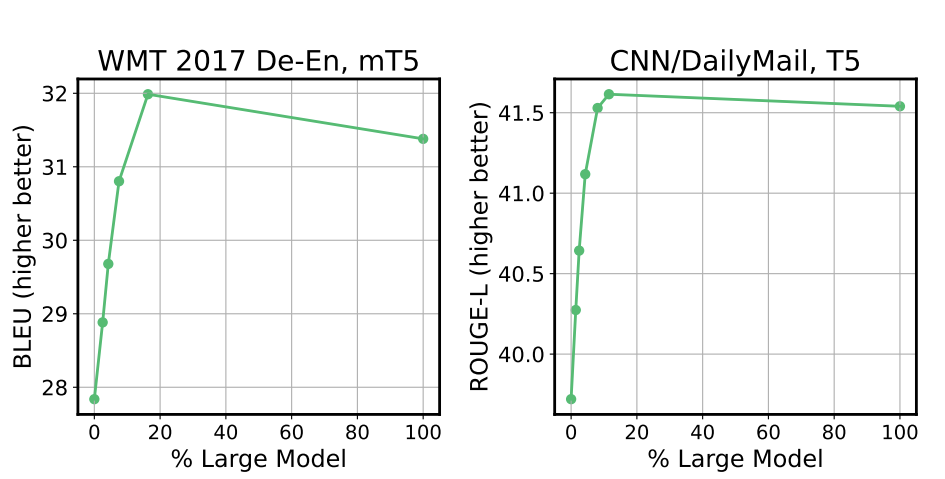
\includegraphics[width=0.6\textwidth]{Motivating.png}
    \caption{
        大模型参与比例的生成质量影响
    }
    \label{fig:Motivating}
\end{figure}

\section{Fallback 策略}

Fallback 策略决定小模型何时将控制权转交给大模型。当小模型对自己的预测不够自信时,让大模型接管预测。信心量化(Confidence Quantification)是一个活跃的研究领域\upcite{gal2016dropout,kendall2017uncertainties},任何轻量级的信心指标都可以作为潜在的候选指标。该文使用最大预测概率量化判别转交时机:当最大预测概率 $\max _y p_S\left(y \mid y_{1: n-1}\right)$ 小于阈值 $\alpha_{FB}$ 时,认为预测不够可信,出错的可能性较高,Fallback 使用大模型生成下一个标记。

\begin{figure}[htbp]
    \centering
    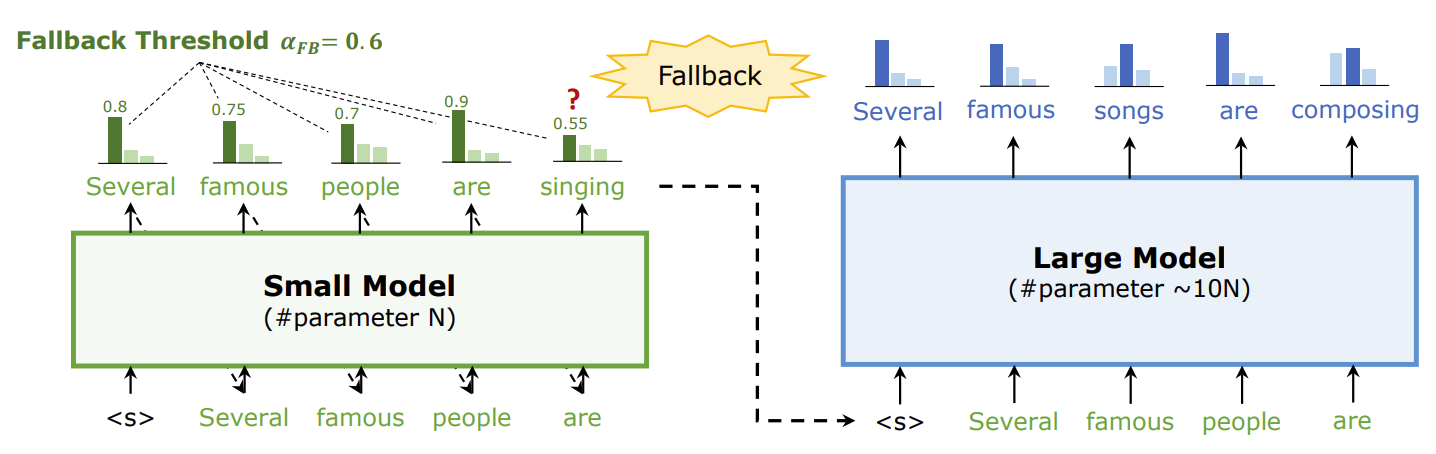
\includegraphics[width=0.9\textwidth]{Fallback.png}
    \caption{
        Fallback 策略:在小模型自回归生成标记时,如果标记的最大预测概率低于阈值 $\alpha_{FB}$ ,则认为预测不够可信,使用大模型生成标记。
    }
    \label{fig:Fallback}
\end{figure}

\section{Rollback 策略}

当小模型对预测结果不够自信,决定使用 Fallback 策略时,它先前的预测可能也是不准确的。早期解码迭代中的一次错误预测会影响所有后续的文本生成,这可能大幅降低生成质量\upcite{schuster2022confident}。因此,大模型需要回顾验证小模型的历史预测,并在必要时予以修正。

对于距离指标 $d(\cdot,\cdot)$(可使用交叉熵函数),寻找大于阈值 $\alpha_{RB}$ 的最小的解码步 $m$,满足

\begin{equation}
    d\left(p_S\left(y \mid y_{1: m}\right), p_L\left(y \mid y_{1: m}\right)\right)>\alpha_{R B}
\end{equation}

如果 $m$ 存在,就认为小模型生成的标记 $y_m$ 是不准确的,Rollback 撤销 $y_{m}$ 和 $y_{n}$ 之间的预测并将 $y_m$ 替换为大模型的预测 $y_{m,L}$。

\begin{figure}[htbp]
    \centering
    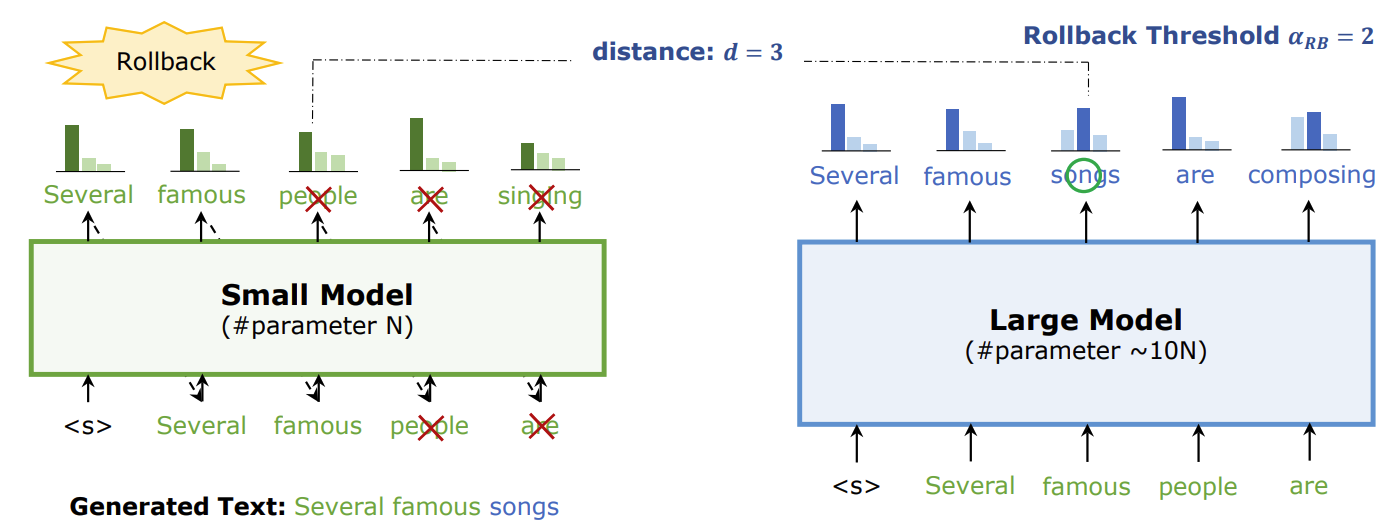
\includegraphics[width=0.9\textwidth]{Rollback.png}
    \caption{
        Rollback 策略:
        当大模型接管控制权时(即 Fallback 策略生效后),它会重新生成之前和当前的所有标记。
        如果大模型和小模型的预测概率差异 $d$ 超过了阈值 $\alpha_{RB}$,则撤销小模型的预测。
    }
    \label{fig:Rollback}
\end{figure}

\section{预测对齐}

如果大模型和小模型的词汇表一致,BiLD 框架对大小模型的选择没有限制。然而,当两个模型分别训练时,他们可能会得到语义相近但是词汇表不同的训练结果。Rollback 策略需要衡量大模型和小模型的标记相似度,语义相近但是词汇不同的标记会造成额外的 Rollback,这样非但不会提升生成质量,还会降低推理速度。

为了对齐小模型和大模型的词汇表,BiLD 可以使用模型对齐技术。在使用数据集训练完大模型后,提取一个能有效表示数据集语句分布的校准数据集 $\mathcal{X}_{\mathrm{cal}}=\{x^{(i)}\}$,使用大模型获取对应的输出 $\mathcal{Y}_{\mathrm{cal}}=\{y^{(i)}\}$。再使用校准集 $\left(x_{\mathrm{cal}}, y_{\mathrm{cal}}\right) \in\left(\mathcal{X}_{\mathrm{cal}}, \mathcal{Y}_{\mathrm{cal}}\right)$ 对小模型进行微调。

这样做可以提升小模型和大模型的预测相似度,降低 Rollback 判断中的距离 $d(\cdot,\cdot)$,从而减少不必要的 Rollback,进一步提升 BiLD 推理速度。

% !Mode:: "TeX:UTF-8"
\chapter{实验分析}

\section{实验过程}

该文选择 WSLT 2017 De-En\upcite{iwslt} 和 WMT 2014 De-En\upcite{wmt} 作为机器翻译数据集,XSUM\upcite{xsum} 和 CNN/DailyMail\upcite{cnn}作为摘要生成数据集。

在模型的选择方面,使用 mT5-large and small\upcite{xue2021mt5} 作为机器翻译模型,使用 T5-large and small \upcite{raffel2023exploring} 作为摘要生成模型。大小模型相差约 20 倍。

该文在对预先训练好的大模型进行 50 万步的微调,从而得到基准的大模型。为了实现预测对齐,先使用完成微调的大型模型从输入数据集 $\mathcal{X}_{\text {cal }}=\left\{x^{(i)}\right\}$ 生成输出序列 $\mathcal{Y}_{\text {cal }}=\left\{y^{(i)}\right\}$,创建校准数据集。然后,使用校准数据集 $\left(x_{\text {cal }}, y_{\text {cal }}\right) \in\left(\mathcal{X}_{\text {cal }}, \mathcal{Y}_{\text {cal }}\right)$ 对小模型进行微调。

推理评估在 GCP n1-standard-4 实例的单个 NVIDIA T4 GPU 上进行。该文对不同的 Fallback 和 Rollback 阈值进行了测试,并分别使用或关闭预测对齐,探究生成质量和延迟的权衡。

\section{实验结果}

通过调整 Fallback 和 Rollback 阈值和是否使用预测对齐,研究文本生成质量与推理速度的关系,主要结果如图~\ref{result} 和表~\ref{result_table} 所示。图表中给出了 Vanilla Inference 基准数据。在消融研究中,分别去除 Fallback 和 Rollback 部分,验证 BiLD 的有效性。

\begin{figure}[htbp]
    \centering
    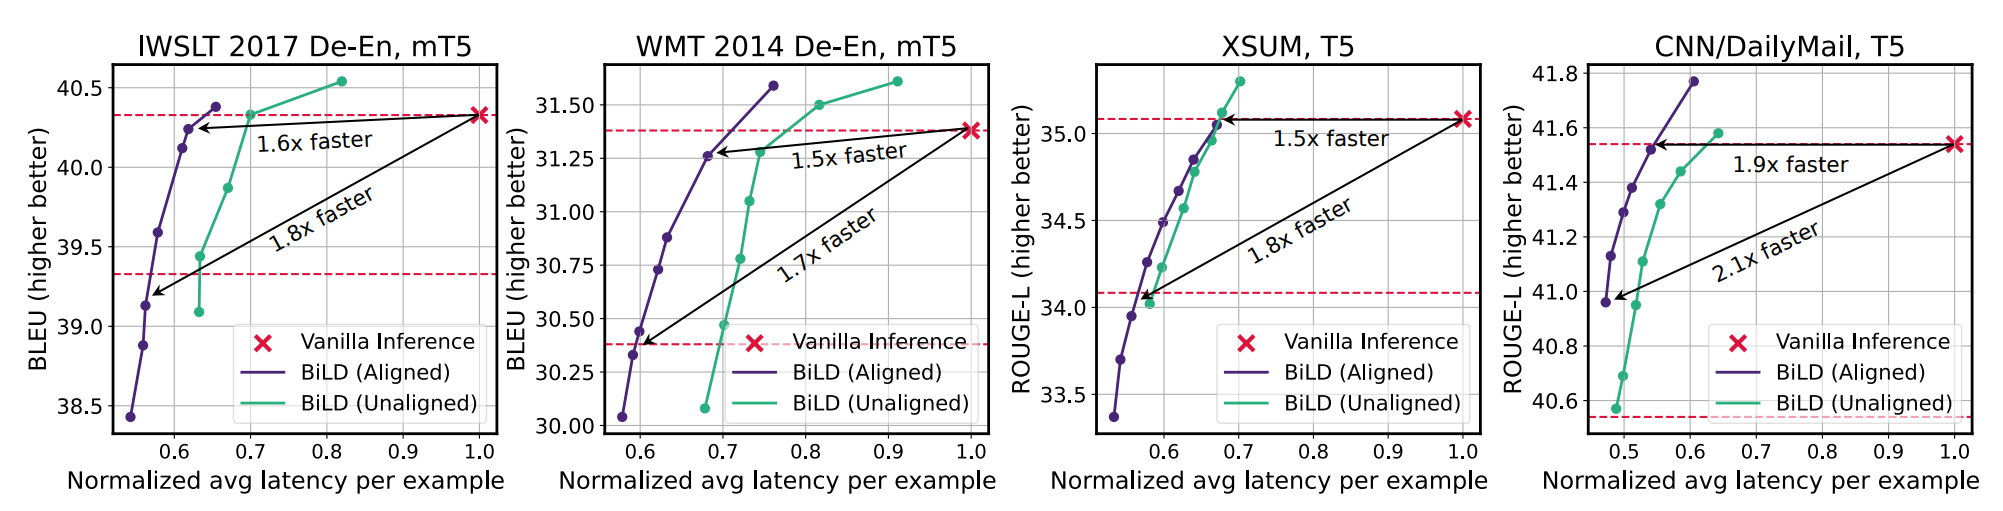
\includegraphics[width=0.9\textwidth]{result.png}
    \caption{实验结果}
    \label{result}
\end{figure}

\begin{table}[htbp]
    \centering
    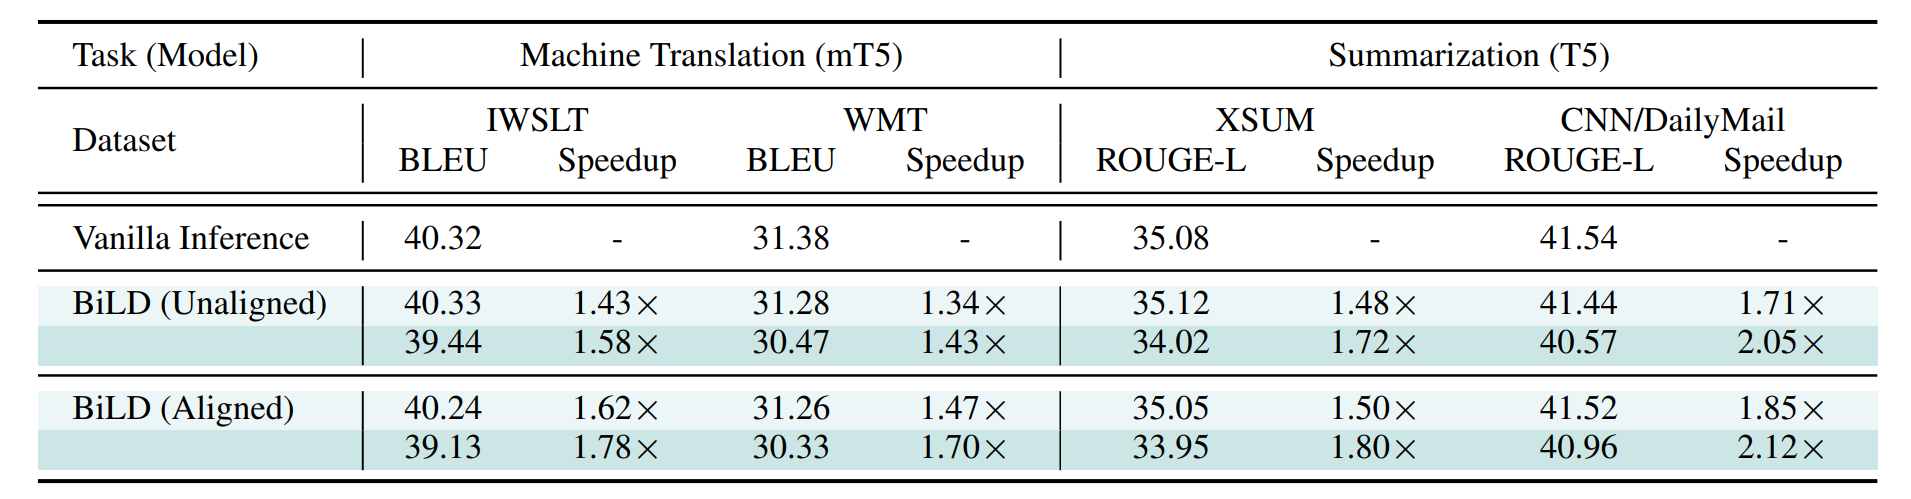
\includegraphics[width=0.9\textwidth]{result_table.png}
    \caption{实验数据总结}
    \label{result_table}
\end{table}
在不进行预测对齐时, BiLD 相对所有基准测试平均提速至 $1.5\sim 2.0$ 倍。未对齐的 BiLD 是一种纯粹的即插即用解决方案,除了独立准备小型模型外,不需要额外的工作。

对齐的 BiLD 比未对齐的 BiLD 有了进一步改进,提速为 $1.6\sim 2.1$ 倍。结果还表明,在允许高延迟时(仍比基准模型快),未对齐和已对齐的 BiLD 都优于基准分数,这可以归因于使用两种不同模型的集合效应\upcite{matsubara2022ensemble}。

\section{消融研究}

分别去除 Rollback 和 Fallback ,研究 BiLD 有效性,结果如图~\ref{ablation}所示。可以发现,尽管 Rollback 回退会造成额外开销,但生成质量的提高更显著。如果取消 Fallback,替换为生成一定数量标记后定期将控制权移交给大模型,会导致性能显著下降。这说明 BiLD 的 Fallback 和 Rollback 策略都是有效的。

\begin{figure}[htbp]
    \centering
    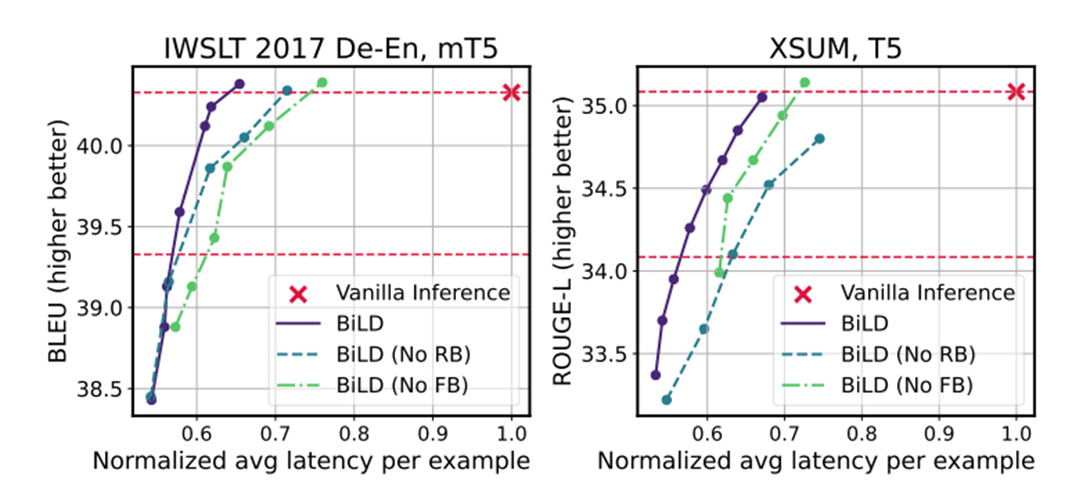
\includegraphics[width=0.9\textwidth]{ablation.png}
    \caption{实验结果}
    \label{ablation}
\end{figure}

% !Mode:: "TeX:UTF-8"
\chapter{论文不足}

尽管 BiLD 无需修改模型架构和训练流水线,但没有说明给定一个大模型,如何有效地选择相应的小模型。并且没有提及大模型和小模型在模型尺度方面应当具有多大的差异。

BiLD 框架需要调整阈值 Fallback $\alpha_{FB}$ 和 Rollback $\alpha_{RB}$,超参数的选取可能因任务和模型而异,文章没有讨论如何搜索这些参数。

该文没有讨论大模型倾向于纠正哪些类型的预测,即大模型和小模型的预测差异的具体表现。

BiLD 仅在机器翻译和文本摘要数据集上进行了评估,这些数据集已被证明对于小型或非自回归模型来说并不困难\upcite{kasai2021deep,gu2019levenshtein}。应该对更具挑战性的数据集进行评估,例如 HumanEval\upcite{chen2023accelerating}。

% !Mode:: "TeX:UTF-8"
\chapter*{结论\markboth{结论}{}}
\addcontentsline{toc}{chapter}{结论}

该文提出了一种新型框架 Big Little Decoder(BiLD),这是一个无需额外训练或修改现有模型就能减少各种文本生成任务的端到端推理延迟的框架。从本质上讲,BiLD 将大小解码器模型结合在一起,从而更高效地生成文本。BiLD 从一个小型模型开始推理,小模型在大部分时间内以自回归方式运行,以较低的推理成本生成文本。而大型模型则以非自回归方式执行,以完善小型模型的不准确预测。BiLD 包含两种策略,一种是 Fallback 策略(当小模型不确定时,将控制权交给大模型),另一种是 Rollback 策略(允许大模型恢复小模型不准确的预测)。BiLD 在机器翻译、摘要和语言建模文本生成场景中进行了评估。在 NVIDIA Titan Xp GPU 上运行时,BiLD 的性能没有下降,平均速度提高为 1.52 倍,在某些任务上达到了 2.18 倍。此外,在允许性能下降 1 点的情况下,BiLD 的平均速度提高了 1.76 倍,某些任务的速度提高了 2.38 倍。总之,该文通过创新性地设计 BiLD 框架,在保持了与现有模型的兼容性的同时,有效地提高了文本生成任务的推理效率,为 NLP 领域的研究和应用提供了有益的思路和方法。


% 致谢
% % !Mode:: "TeX:UTF-8"
% \chapter*{致谢}
% \addcontentsline{toc}{chapter}{致谢}
% %此处致谢内容
% \cleardoublepage

% 参考文献
\include{data/reference}

% 附录
\appendix
% % !Mode:: "TeX:UTF-8"
% \chapter{常见问题}
% \label{chapter-faq}
% \begin{enumerate}
% \item 本模板如何使用?
% \label{faq-howtouse}
% \begin{itemize}
%     \item 按照第2章的要求,先下载和安装相应的软件,推荐使用\TeX{}Live;
%     \item 下载cls文件;
%     \item 使用tex的编辑器或其他编辑器,编写论文,注意保存为UTF-8编码;
%     \item xelatex编译。
% \end{itemize}
% \item Windows下的msmake.bat如何使用?
% \label{faq-msmake}
% \begin{itemize}
%     \item 使用Windows的CMD命令行,进入到msmake.bat所在目录;
%     \item 键入~msmake~后会显示相应的帮助文件;
%     \item 按照所显示的相关信息再键入相应命令即可。
% \end{itemize}
% \item 使用TexLive如何更新?
% \label{faq-texliveupdate}
% TUG官方推荐\TeX{}Live通过镜像站进行更新,具体步骤为:
% \begin{itemize}
%     \item 在“开始”菜单中,找到有TeX Live Manage程序;
%     \item 在菜单“tlmgr”下选择“载入其他仓库”,选择最近的仓库即可(如果是北航校内用户并能够
%     访问到\href{http://mirror.buaa.edu.cn/}{北航开源镜像站}的话,可以在仓库地址中
%     输入\texttt{http://mirror.buaa.edu.cn/CTAN/systems/texlive/tlnet/});
%     \item 按照目录选择更新。
% \end{itemize}
% \end{enumerate}

% % !Mode:: "TeX:UTF-8"
% \chapter{联系我们}

\end{document}
